\section{Problem D}
    \subsection{Statement}
        \href{http://foobar.iiitd.edu.in/contest/team/problem.php?id=530}{click}

    \subsection{Solution}
        The key idea of the solution is the Inclusion Exclusion Principle.
        We will demonstrate the idea visually.
        Consider this image
        \marginpar{all images made using \href{https://www.geogebra.org}{geogebra}}, corresponding to the input
        \begin{verbatim}
            3
            5 3 4
            6 4 3
            7 1 6
        \end{verbatim}

        \begin{center}
            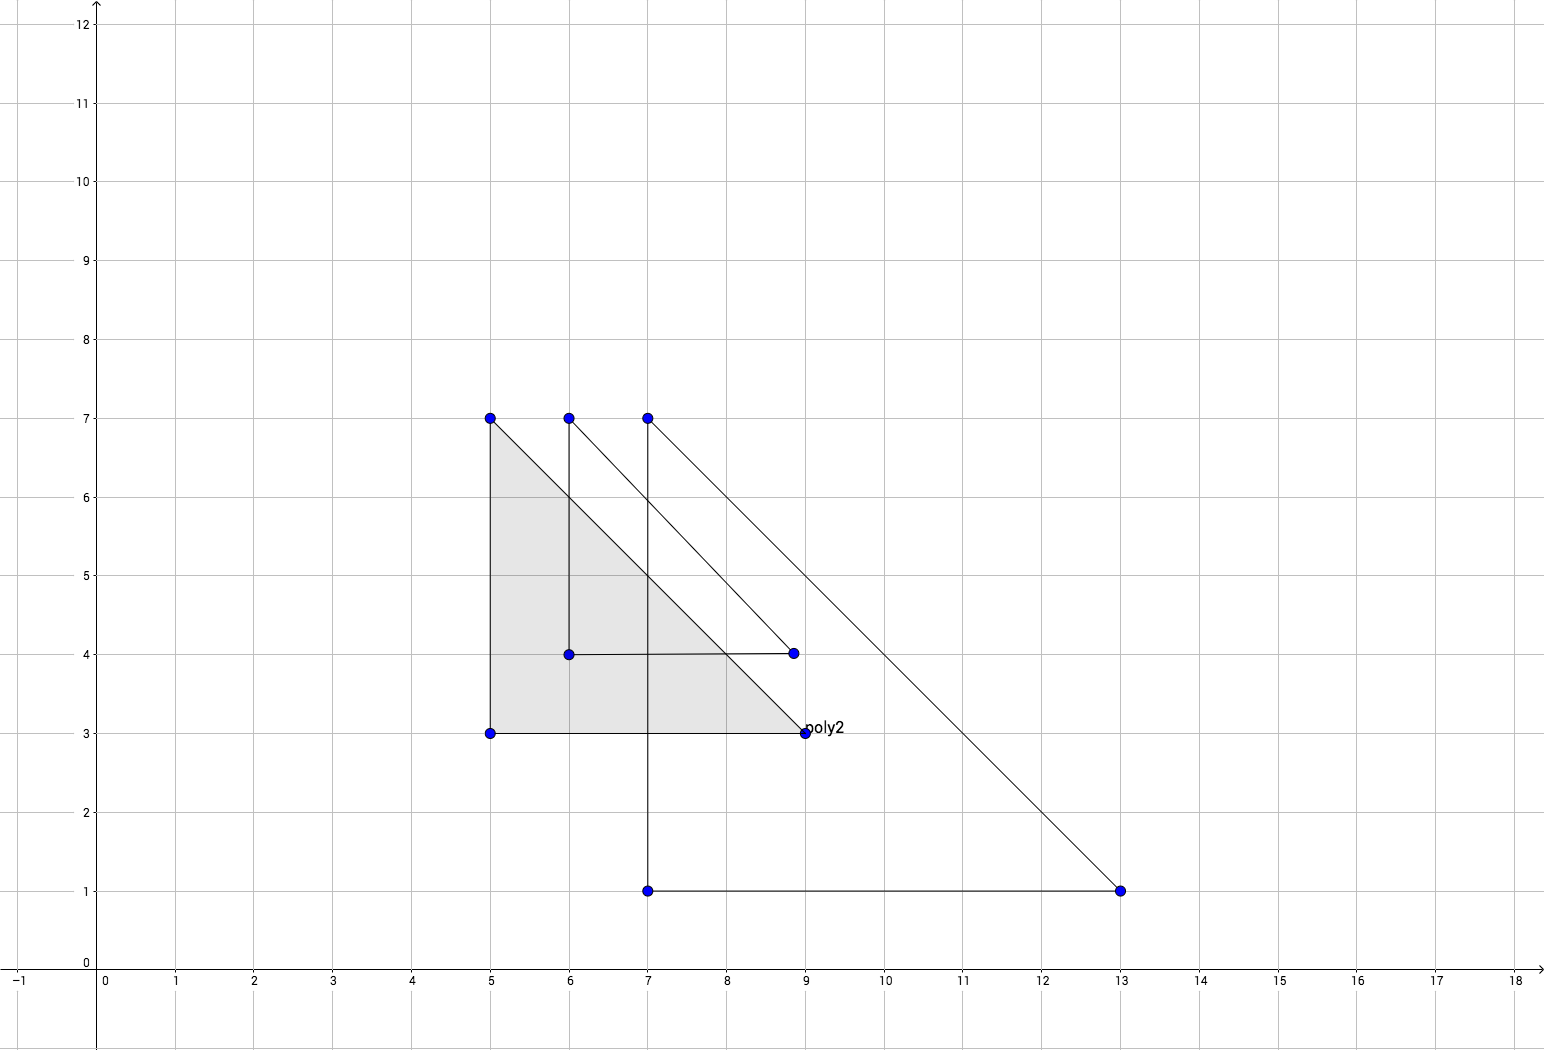
\includegraphics[scale=0.2]{images/input.png}
        \end{center}

        First, we note that any point that belongs to exactly an odd number of triangles
        is coloured black, everything else is white.
        So to count such areas, first we \emph{include} all the areas which belong to
        \emph{at least} one triangle, like so

        \begin{center}
            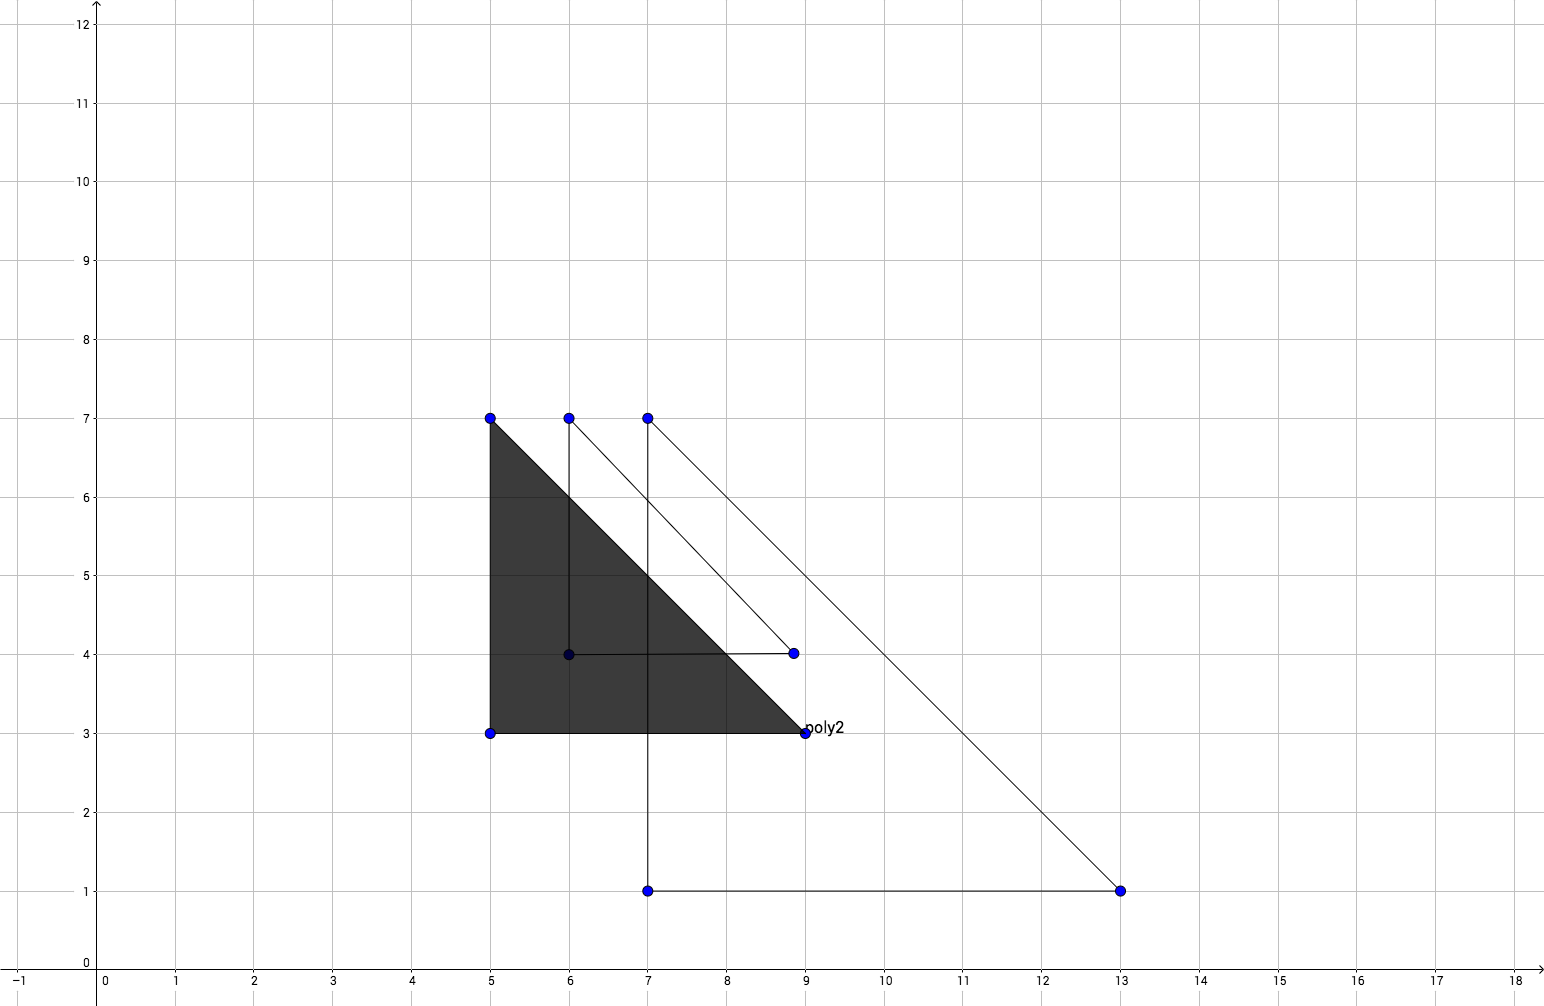
\includegraphics[scale=0.1]{images/color1.png}
            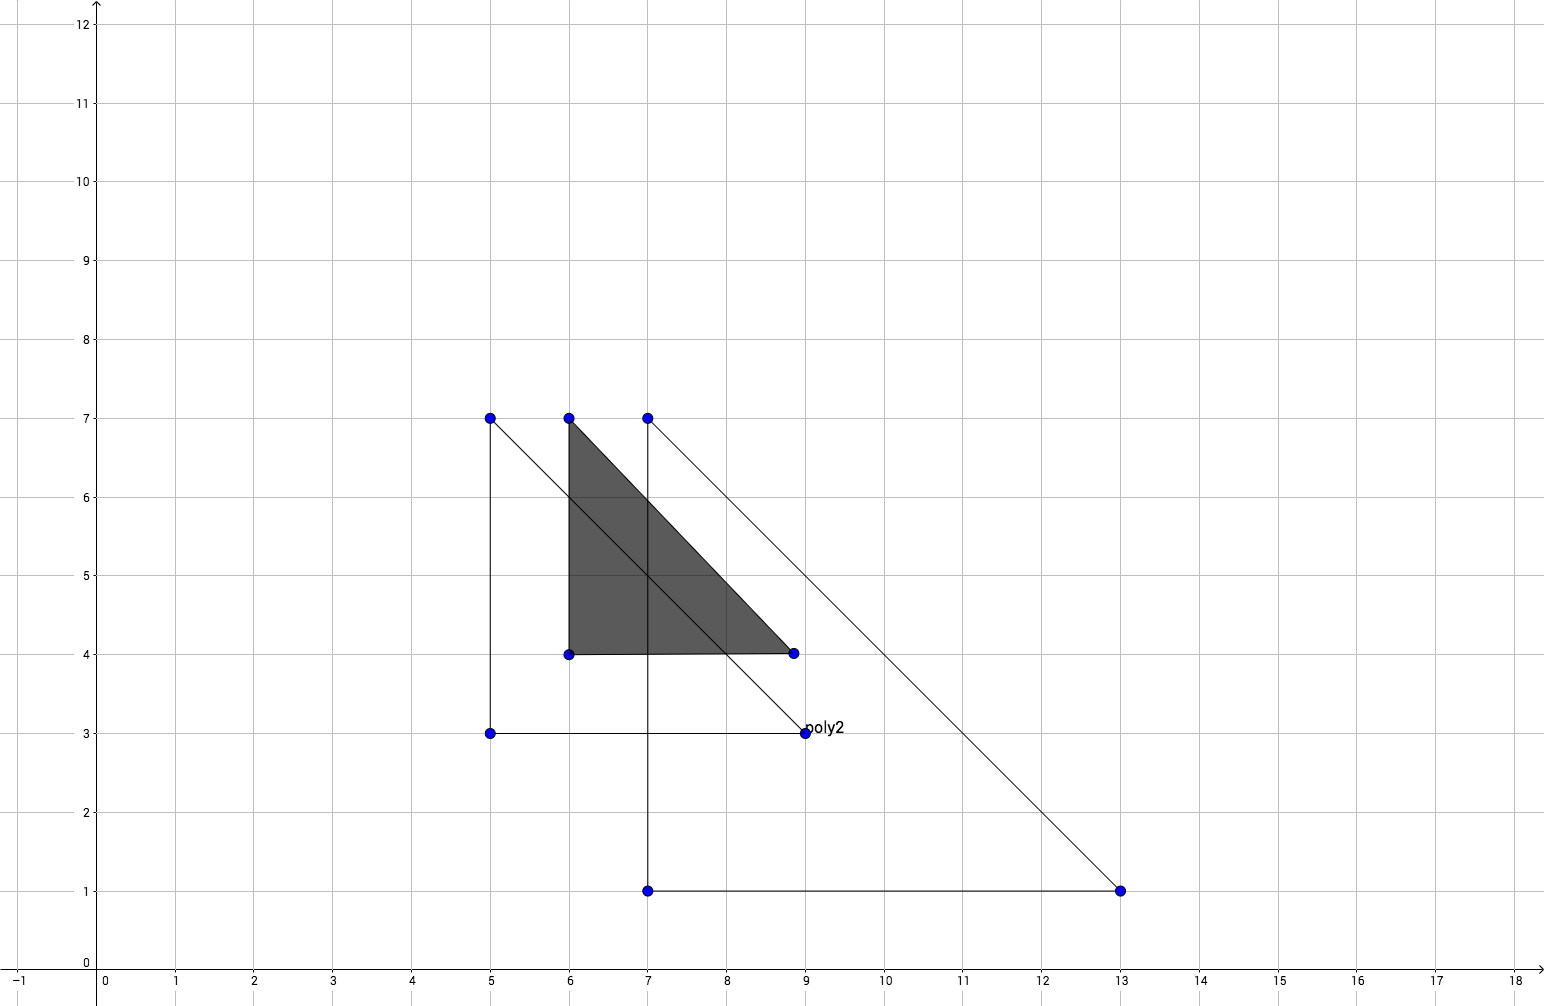
\includegraphics[scale=0.1]{images/color2.png}
            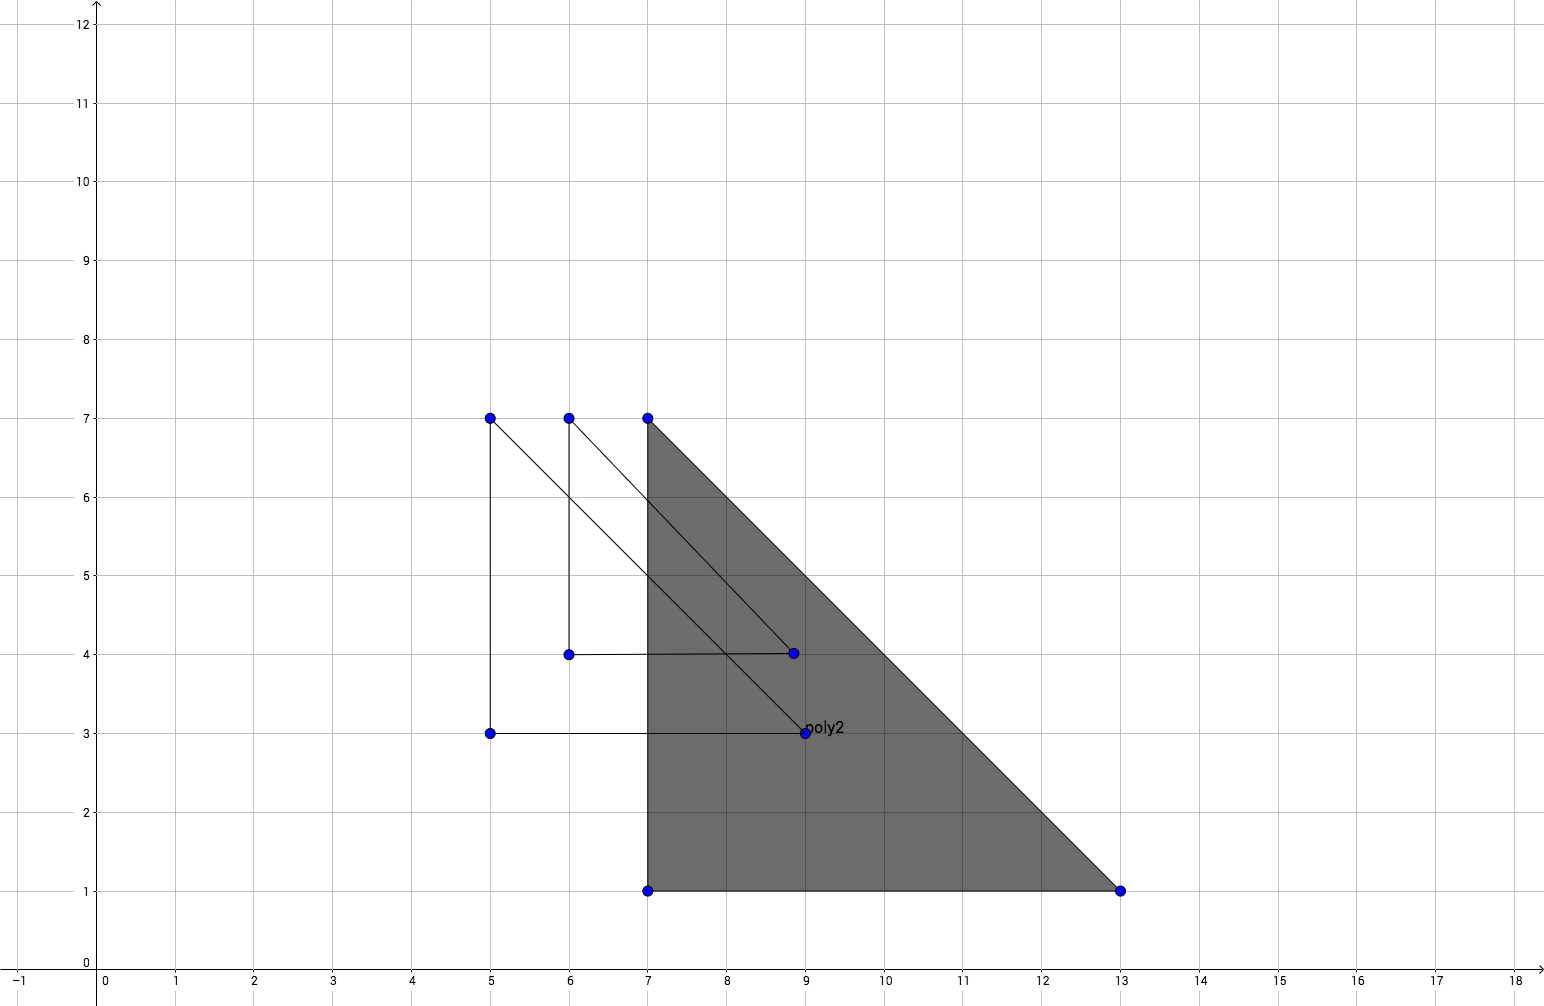
\includegraphics[scale=0.1]{images/color4.png}
        \end{center}

        But now it appears that by having the rather relaxed approach to counting we
        started with, we have
        \begin{itemize}
            \item counted the points inside exactly two triangles (and twice, scandalous),
            whereas they are not meant to be counted at all.
            \item counted the points inside all three triangles thrice (!).
        \end{itemize}

        So in the next phase, we \emph{exclude} any point which belongs to \emph{at least}
        two triangles, like so

        \begin{center}
            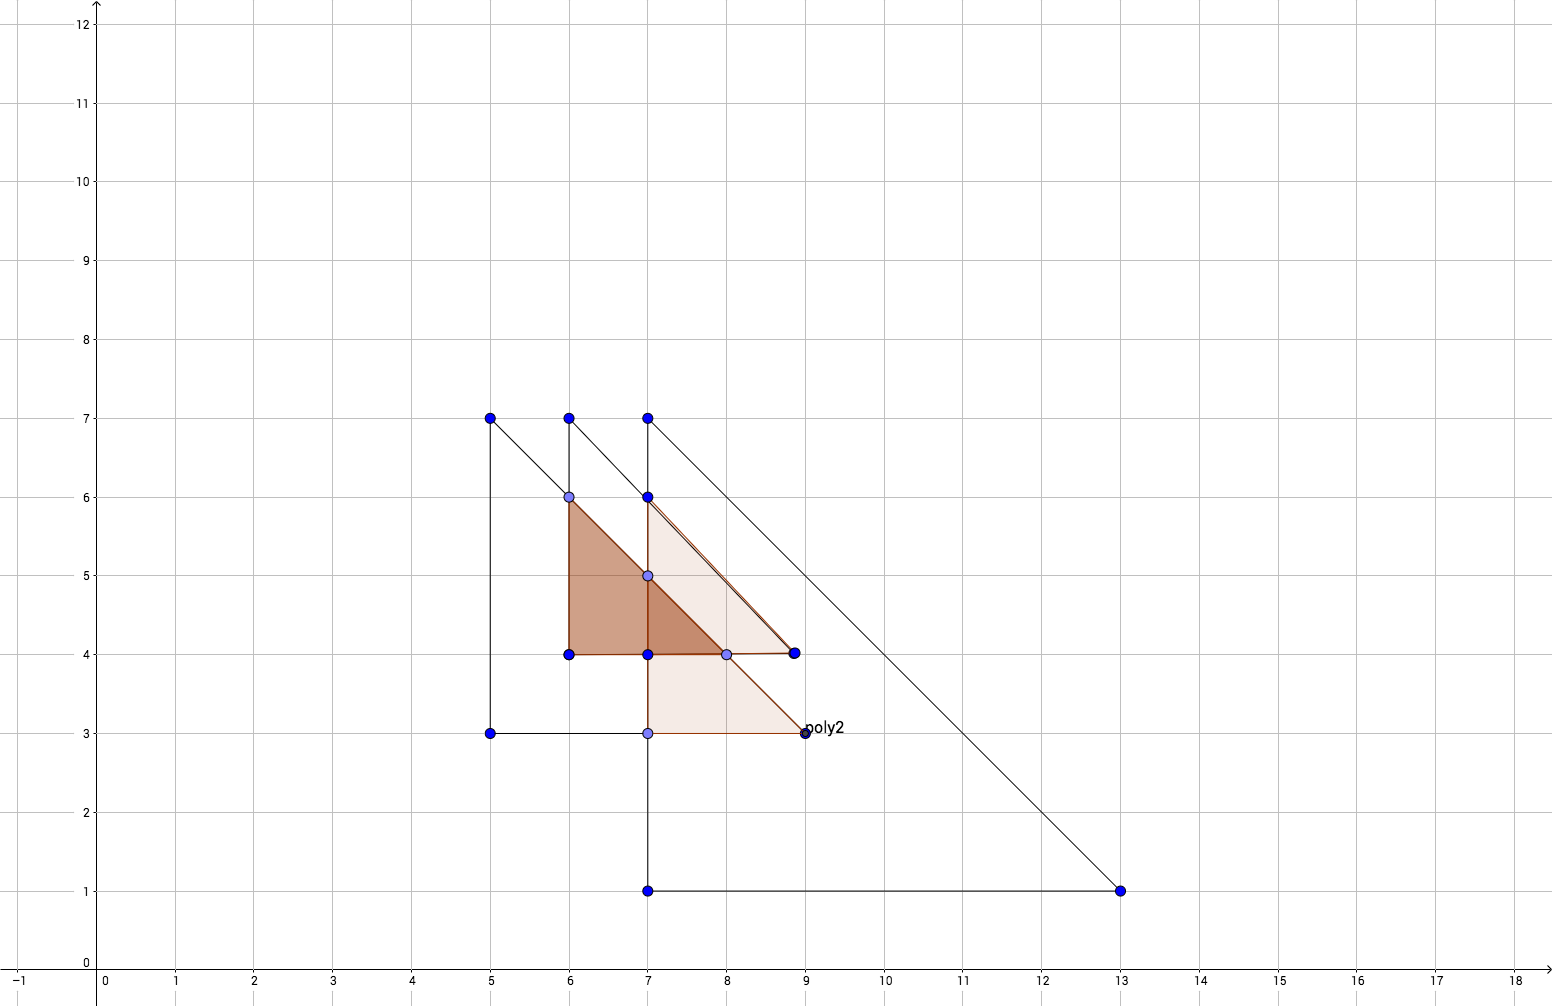
\includegraphics[scale=0.1]{images/color3.png}
            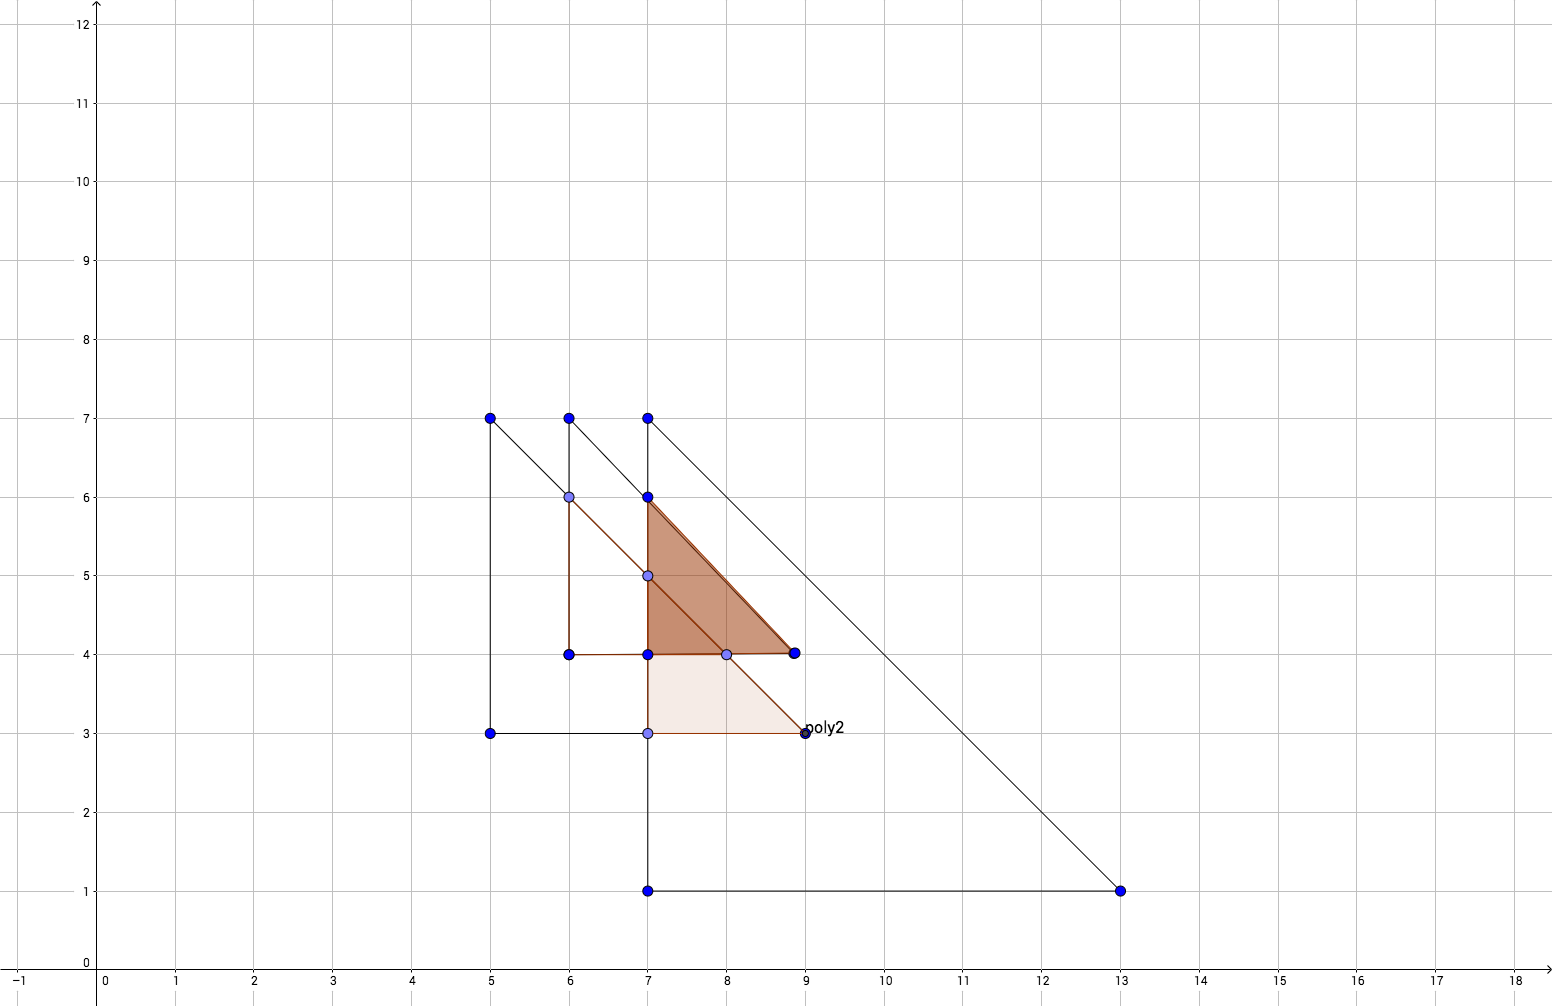
\includegraphics[scale=0.1]{images/color6.png}
            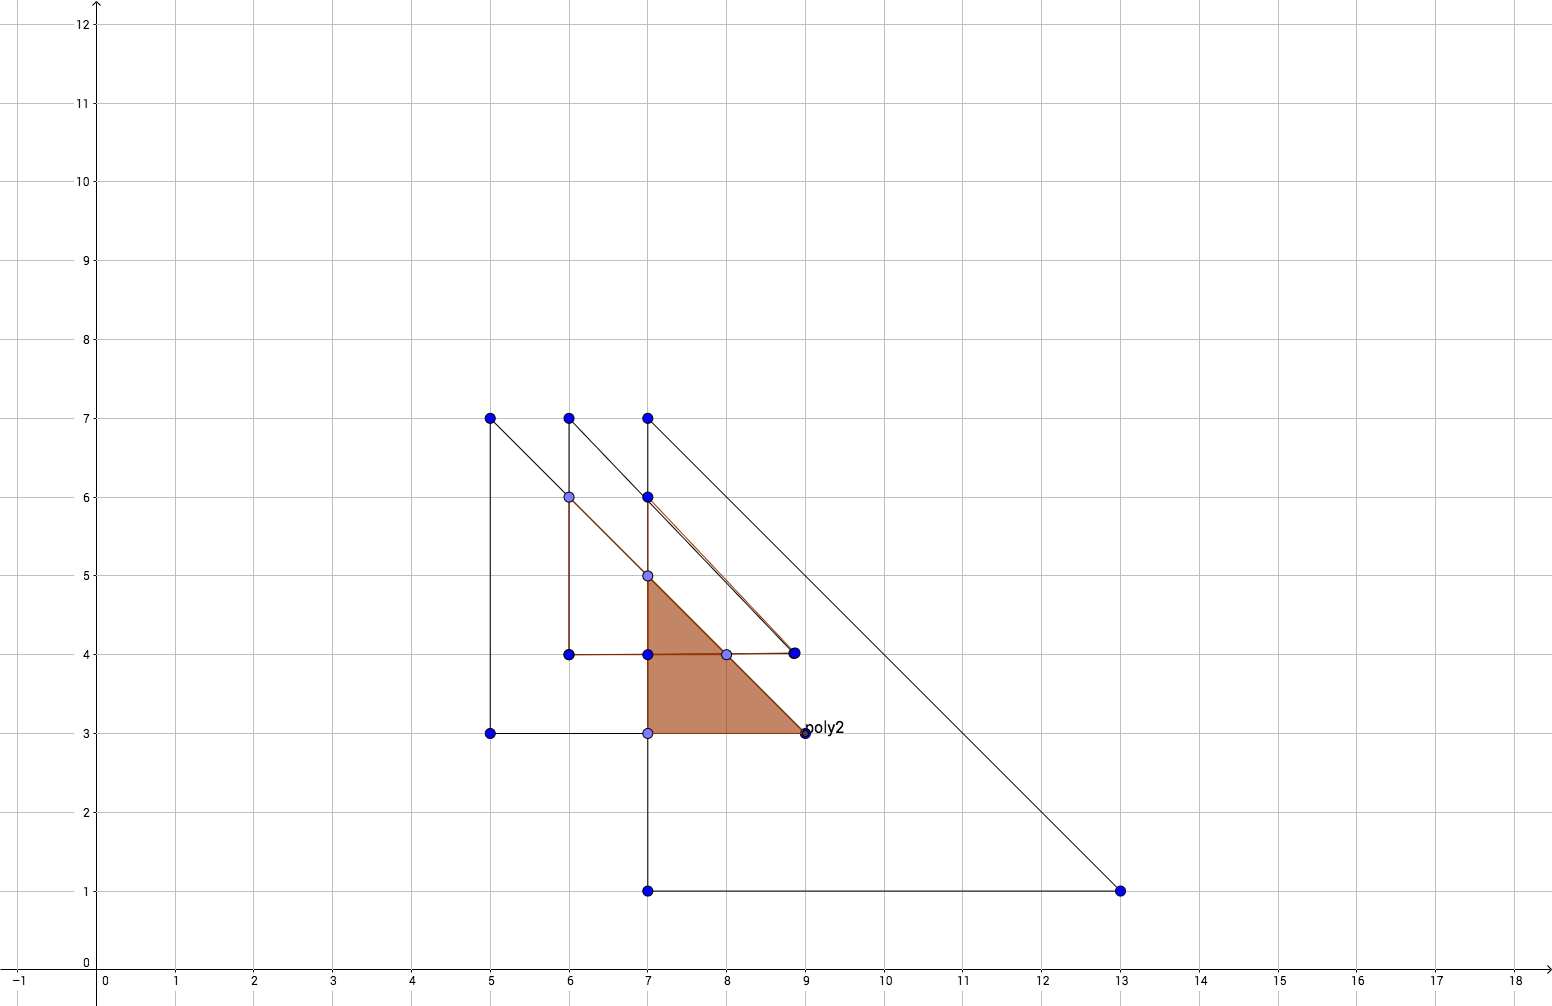
\includegraphics[scale=0.1]{images/color5.png}
        \end{center}

        But wait, we added them twice (remember?), so we need to subtract each of them twice.
        So now it appears we've got everything worked out, except

        \begin{itemize}
            \item subtracted the points inside all three triangles 6 times after adding them thrice.
            remember that since these points are inside 3 (an odd number) triangles, we need to add them
            once.
        \end{itemize}

        So we now \emph{include} the points which are inside at least $3$ triangles $4$ times

        \begin{center}
            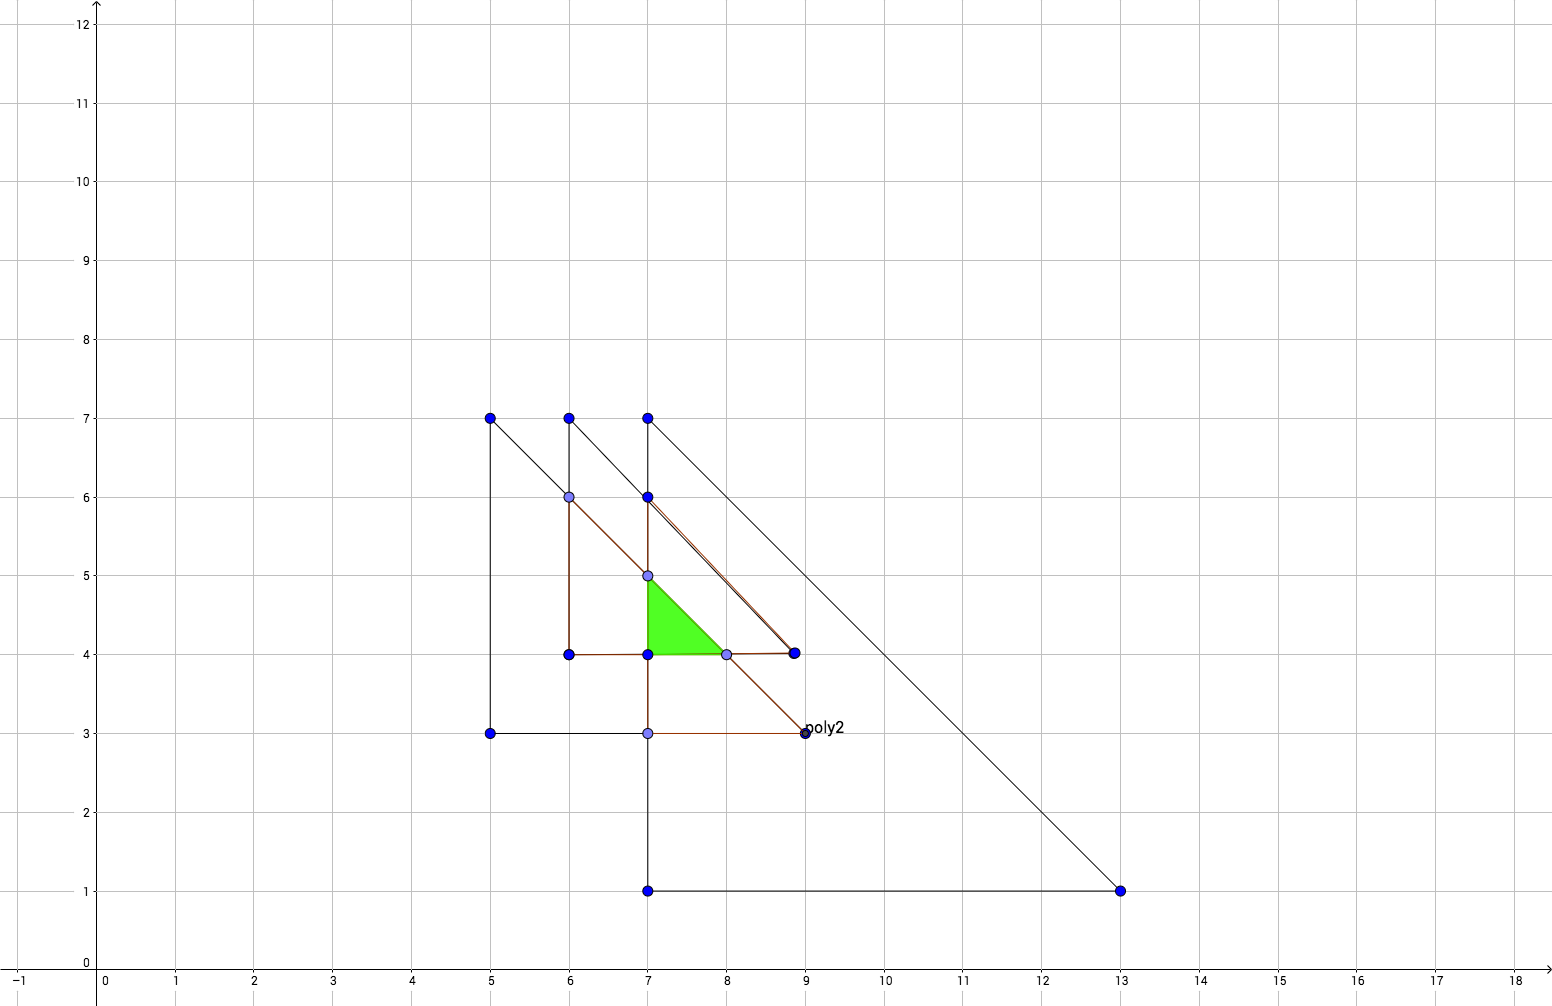
\includegraphics[scale=0.2]{images/color7.png}
        \end{center}

        Now it finally looks like we're good.

        So, what is the general approach while using the Inclusion-Exlusion Principle?
        Note that initially, we wanted to count points which are inside \emph{exactly} $K$ triangles,
        and that seems quite hard. Instead, if we are clever, it is enough to have the ability to
        count the points inside \emph{at least} $K$ triangles, which turns out to be much easier
        (as we will see).
        
        As an exercise, try to solve this:
        If two sets $H$ and $G$ have cardinalities $|H|$ and $|G|$ respectively, then, what is the
        number of surjections from $H$ to $G$?

        Now, back to our problem. It seems that we now have two things left to do.
        \begin{itemize}
            \item find the intersection of an arbitrary number of axis aligned right isosceles triangles
            \item enumerate all possible subsets of a set. If you turn back the pages, you'll see this is
            exactly what we (stealthily) did, and note that we're applying a scaling factor of $(-2)^{K - 1}$
            on a subset of size $K$. So if you could enumerate all subsets of the input set of triangles,
            combined with the previous point you have a complete algorithm.
        \end{itemize}

        Due to the limited time and typesetting skill of yours truly, these two loose ends are left as
        an exercise.
        The first one is mostly trivial geometry (hint: the intersection of two axis aligned right isosceles triangles
        gives another axis aligned right isosceles triangle).
        For the second one, it serves well to know either \verb|recursion|, or \verb|python|, or \verb|bitmasks|.
